%!TEX TS-program = xelatex
\documentclass[10pt, compress]{beamer}

\usetheme[usetitleprogressbar]{m}

\usepackage[export]{adjustbox}
\usepackage{etoolbox}
\usepackage{booktabs}
\usepackage{dcolumn}
\usepackage[scale=2]{ccicons}
\usepackage{color}

% math typesetting
\usepackage{array}
\usepackage{amsmath}
\usepackage{amssymb}
\usepackage{amsthm}
\usepackage{amsfonts}
\usepackage{relsize}
\usepackage{mathtools}
\usepackage{bm}

% tables
\usepackage{tabularx}
\usepackage{booktabs}
\usepackage{multicol}
\usepackage{multirow}
\usepackage{colortbl}

% graphics stuff
\usepackage{subfig}
\usepackage{graphicx}
\usepackage[space]{grffile} % allows us to specify directories that have spaces
\usepackage{tikz}

% to change enumeration symbols begin{enumerate}[(a)]
\usepackage{enumerate}

% Add some colors
\definecolor{red1}{RGB}{253,219,199}
\definecolor{red2}{RGB}{244,165,130}
\definecolor{red3}{RGB}{178,24,43}

\definecolor{green1}{RGB}{229,245,224}
\definecolor{green2}{RGB}{161,217,155}
\definecolor{green3}{RGB}{49,163,84}

\definecolor{blue0}{RGB}{255,247,251}
\definecolor{blue1}{RGB}{222,235,247}
\definecolor{blue2}{RGB}{158,202,225}
\definecolor{blue3}{RGB}{49,130,189}
\definecolor{blue4}{RGB}{4,90,141}

\definecolor{purple1}{RGB}{191,211,230}
\definecolor{purple2}{RGB}{140,150,198}
\definecolor{purple3}{RGB}{140,107,177}

\definecolor{brown1}{RGB}{246,232,195}
\definecolor{brown2}{RGB}{223,194,125}
\definecolor{brown3}{RGB}{191,129,45}

% square bracket matrices
\let\bbordermatrix\bordermatrix
\patchcmd{\bbordermatrix}{8.75}{4.75}{}{}
\patchcmd{\bbordermatrix}{\left(}{\left[}{}{}
\patchcmd{\bbordermatrix}{\right)}{\right]}{}{}

% easy command for boldface math symbols
\newcommand{\mbs}[1]{\boldsymbol{#1}}

% command for R package font
\newcommand{\pkg}[1]{{\fontseries{b}\selectfont #1}}

% approx iid
\newcommand\simiid{\stackrel{\mathclap{\normalfont\mbox{\tiny{iid}}}}{\sim}}

% references to graphics
\makeatletter
\def\input@path{{/Users/janus829/Research/netsMatter/prezzy/graphics/}, {/Users/s7m/Research/netsMatter/prezzy/graphics/}}
\graphicspath{{/Users/janus829/Research/netsMatter/prezzy/graphics/}, {/Users/s7m/Research/netsMatter/prezzy/graphics/}}

\title[AMEN]{\textsc{Taking Dyads Seriously}}
\author[Minhas et al.]{Shahryar Minhas, Cassy Dorff, Max Gallop, Margaret Foster, Juan Tellez, Howard Liu, Michael Ward} 

\date{\today}

\begin{document}
\frame{\titlepage}

%%%%%%%%%%%%%%%%%%%%%%%%%%%%%%%%%%%%%%%%%%%%%%%%%%%%%%%%%%%%
\frame{
  \frametitle{Motivation}

  \vspace{-10mm}
  Much of international relations data consists of
  \begin{itemize}
    \item a set of units or nodes
    \item a set of measurements, $y_{ij}$, specific to pairs of nodes $(i,j)$ 
  \end{itemize}

  \centering
  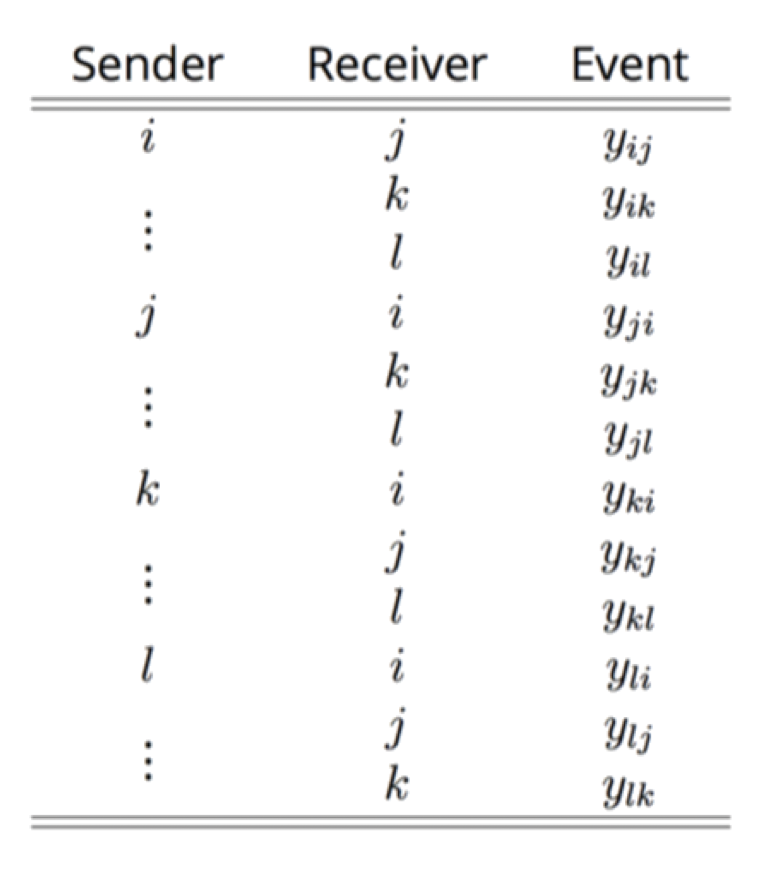
\includegraphics[width=.5\textwidth]{dyadDF}
}
%%%%%%%%%%%%%%%%%%%%%%%%%%%%%%%%%%%%%%%%%%%%%%%%%%%%%%%%%%%%

%%%%%%%%%%%%%%%%%%%%%%%%%%%%%%%%%%%%%%%%%%%%%%%%%%%%%%%%%%%%
\frame{
  \frametitle{Relational data assumptions}

GLM: $y_{ij} \sim \beta^{T} X_{ij} + e_{ij}$

Networks typically show evidence against independence of {$e_{ij} : i \neq j$}

Not accounting for dependence can lead to:

\begin{itemize}
\item biased effects estimation
\item uncalibrated confidence intervals
\item poor predictive performance
\item inaccurate description of network phenomena
\end{itemize}

We've been hearing this concern for decades now:

\begin{tabular}{lll}
Thompson \& Walker (1982) & Beck et al. (1998) & Snijders (2011) \\
Frank \& Strauss (1986) & Signorino (1999) & Erikson et al. (2014) \\
Kenny (1996) & Li \& Loken (2002) & Aronow et al. (2015) \\
\end{tabular}

}
%%%%%%%%%%%%%%%%%%%%%%%%%%%%%%%%%%%%%%%%%%%%%%%%%%%%%%%%%%%%

%%%%%%%%%%%%%%%%%%%%%%%%%%%%%%%%%%%%%%%%%%%%%%%%%%%%%%%%%%%%
\frame{
  \frametitle{Outline}

The approach that we will discuss here to deal with dependencies is the Additive and Multiplicative Effects (AME) model (Hoff 2015; Minhas, Hoff \& Ward 2018)

\begin{itemize}
  \item Nodal and dyadic dependencies in networks
  \begin{itemize}
	  \item Can model using the ``A'' in AME
  \end{itemize}
  \item Third order dependencies
  \begin{itemize}
	  \item Can model using the ``M'' in AME
  \end{itemize}
  \item Simulation
  \item Empirical Application
\end{itemize}

}
%%%%%%%%%%%%%%%%%%%%%%%%%%%%%%%%%%%%%%%%%%%%%%%%%%%%%%%%%%%%

%%%%%%%%%%%%%%%%%%%%%%%%%%%%%%%%%%%%%%%%%%%%%%%%%%%%%%%%%%%%
\frame{
  \frametitle{Dependencies in relational data}

  \vspace{-10mm}
  To start to think about dependencies that arise in relational data ...
  \vspace{5mm}

  \centering
  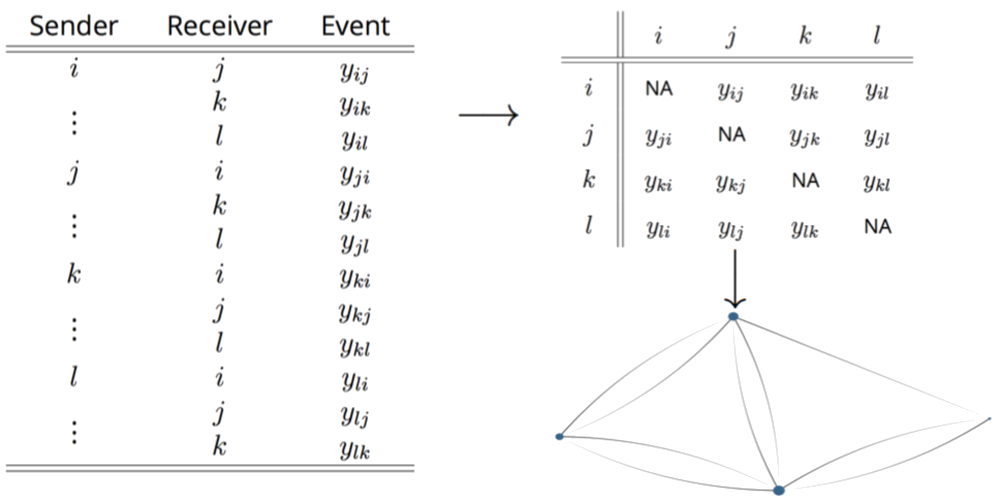
\includegraphics[width=1.05\textwidth]{df_adj_net3}
}
%%%%%%%%%%%%%%%%%%%%%%%%%%%%%%%%%%%%%%%%%%%%%%%%%%%%%%%%%%%%

%%%%%%%%%%%%%%%%%%%%%%%%%%%%%%%%%%%%%%%%%%%%%%%%%%%%%%%%%%%%
\frame{
  \frametitle{What network phenomena? Sender heterogeneity}

  Values across a row, say $\{y_{ij},y_{ik},y_{il}\}$, may be more similar to each other than other values in the adjacency matrix because each of these values has a common sender $i$

  \centering
  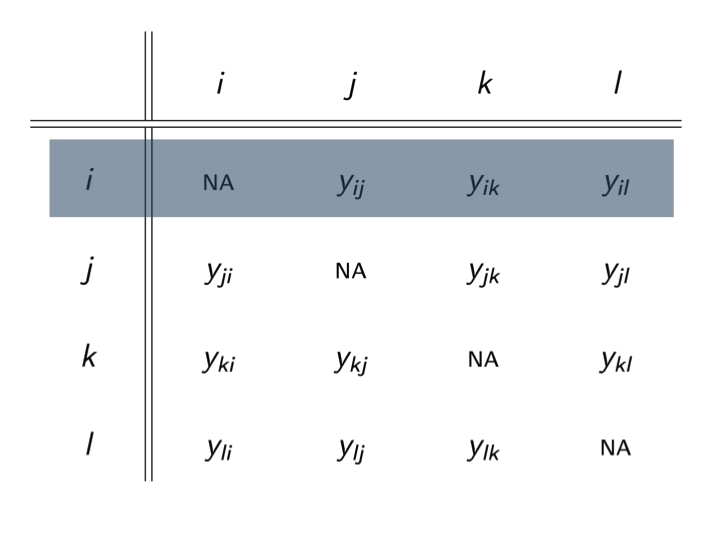
\includegraphics[width=.7\textwidth]{adjRowDep}

}
%%%%%%%%%%%%%%%%%%%%%%%%%%%%%%%%%%%%%%%%%%%%%%%%%%%%%%%%%%%%

%%%%%%%%%%%%%%%%%%%%%%%%%%%%%%%%%%%%%%%%%%%%%%%%%%%%%%%%%%%%
\frame{
  \frametitle{What network phenomena? Receiver heterogeneity}

  Values across a column, say $\{y_{ji},y_{ki},y_{li}\}$, may be more similar to each other than other values in the adjacency matrix because each of these values has a common receiver $i$

  \centering
  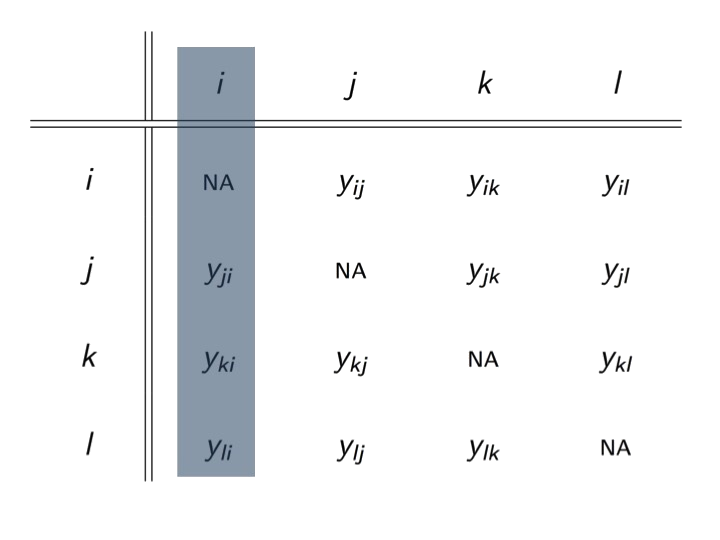
\includegraphics[width=.7\textwidth]{adjColDep}

}
%%%%%%%%%%%%%%%%%%%%%%%%%%%%%%%%%%%%%%%%%%%%%%%%%%%%%%%%%%%%

%%%%%%%%%%%%%%%%%%%%%%%%%%%%%%%%%%%%%%%%%%%%%%%%%%%%%%%%%%%%
\frame{
  \frametitle{What network phenomena? Sender-Receiver Covariance}

  Actors who are more likely to send ties in a network may also be more likely to receive them

  \centering
  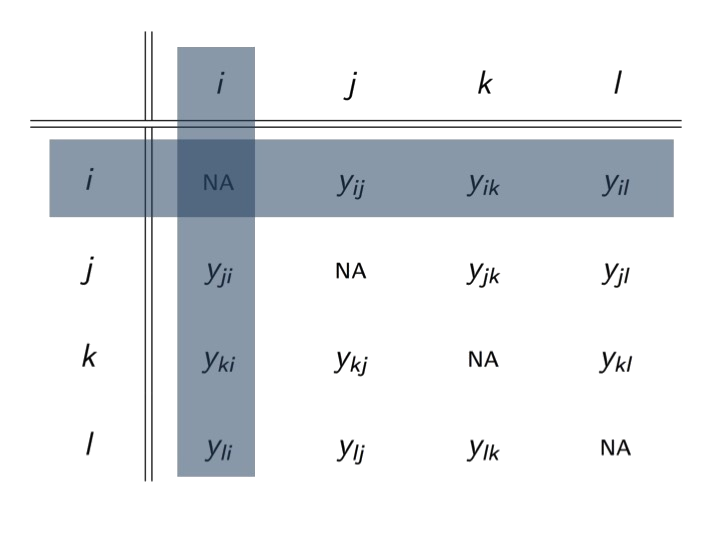
\includegraphics[width=.7\textwidth]{adjRowColCovar}

}
%%%%%%%%%%%%%%%%%%%%%%%%%%%%%%%%%%%%%%%%%%%%%%%%%%%%%%%%%%%%

%%%%%%%%%%%%%%%%%%%%%%%%%%%%%%%%%%%%%%%%%%%%%%%%%%%%%%%%%%%%
\frame{
  \frametitle{What network phenomena? Reciprocity}

  Values of $y_{ij}$ and $y_{ji}$ may be statistically dependent

  \centering
  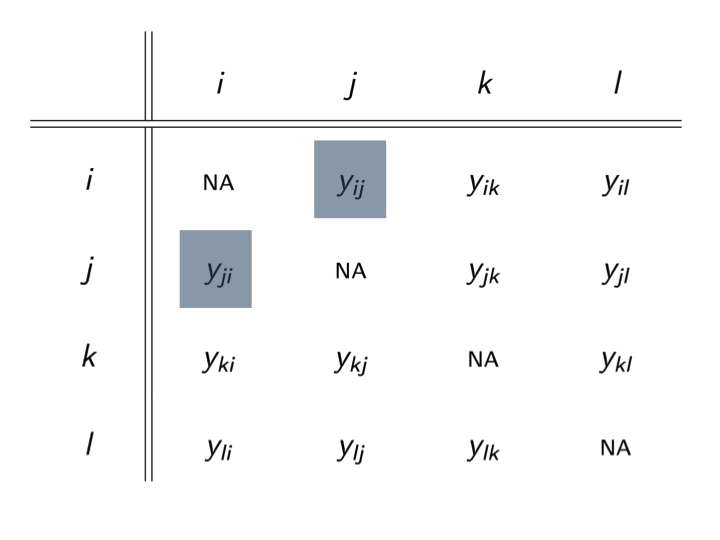
\includegraphics[width=.7\textwidth]{adjRecip}

}
%%%%%%%%%%%%%%%%%%%%%%%%%%%%%%%%%%%%%%%%%%%%%%%%%%%%%%%%%%%%

%%%%%%%%%%%%%%%%%%%%%%%%%%%%%%%%%%%%%%%%%%%%%%%%%%%%%%%%%%%%
\frame{
  \frametitle{Social Relations Model (The ``A'' in AME)}

We use this model to form the additive effects portion of AME (Warner et al. 1979, Li \& Loken 2002, Hoff 2005):

\begin{align*}
\begin{aligned}
      y_{ij} &= \color{red}{\mu} + \color{red}{e_{ij}} \\
      e_{ij} &= a_{i} + b_{j} + \epsilon_{ij} \\
      \{ (a_{1}, b_{1}), \ldots, (a_{n}, b_{n}) \} &\sim N(0,\Sigma_{ab}) \\ 
      \{ (\epsilon_{ij}, \epsilon_{ji}) : \; i \neq j\} &\sim N(0,\Sigma_{\epsilon}), \text{ where } \\
      \Sigma_{ab} = \begin{pmatrix} \sigma_{a}^{2} & \sigma_{ab} \\ \sigma_{ab} & \sigma_{b}^2   \end{pmatrix} \;\;\;\;\; &\Sigma_{\epsilon} = \sigma_{\epsilon}^{2} \begin{pmatrix} 1 & \rho \\ \rho & 1  \end{pmatrix}
\end{aligned}
\end{align*}

\begin{itemize}
\item - $\mu$ baseline measure of network activity
\item - $e_{ij}$ residual variation that we will use the SRM to decompose
\end{itemize}

}
%%%%%%%%%%%%%%%%%%%%%%%%%%%%%%%%%%%%%%%%%%%%%%%%%%%%%%%%%%%%

%%%%%%%%%%%%%%%%%%%%%%%%%%%%%%%%%%%%%%%%%%%%%%%%%%%%%%%%%%%%
\frame{
  \frametitle{Social Relations Model (The ``A'' in AME)}

\begin{align*}
\begin{aligned}
      y_{ij} &= \mu + e_{ij} \\
      e_{ij} &= \color{red}{a_{i} + b_{j}} + \epsilon_{ij} \\
      \color{red}{\{ (a_{1}, b_{1}), \ldots, (a_{n}, b_{n}) \}} &\sim N(0,\Sigma_{ab}) \\ 
      \{ (\epsilon_{ij}, \epsilon_{ji}) : \; i \neq j\} &\sim N(0,\Sigma_{\epsilon}), \text{ where } \\
      \Sigma_{ab} = \begin{pmatrix} \sigma_{a}^{2} & \sigma_{ab} \\ \sigma_{ab} & \sigma_{b}^2   \end{pmatrix} \;\;\;\;\; &\Sigma_{\epsilon} = \sigma_{\epsilon}^{2} \begin{pmatrix} 1 & \rho \\ \rho & 1  \end{pmatrix}
\end{aligned}
\end{align*}

\begin{itemize}
\item - row/sender effect ($a_{i}$) \& column/receiver effect ($b_{j}$)
\item - Modeled jointly to account for correlation in how active an actor is in sending and receiving ties
\end{itemize}

}
%%%%%%%%%%%%%%%%%%%%%%%%%%%%%%%%%%%%%%%%%%%%%%%%%%%%%%%%%%%%

%%%%%%%%%%%%%%%%%%%%%%%%%%%%%%%%%%%%%%%%%%%%%%%%%%%%%%%%%%%%
\frame{
  \frametitle{Social Relations Model (The ``A'' in AME)}

\begin{align*}
\begin{aligned}
      y_{ij} &= \mu + e_{ij} \\
      e_{ij} &= a_{i} + b_{j} + \epsilon_{ij} \\
      \{ (a_{1}, b_{1}), \ldots, (a_{n}, b_{n}) \} &\sim N(0,\color{red}{\Sigma_{ab}}) \\ 
      \{ (\epsilon_{ij}, \epsilon_{ji}) : \; i \neq j\} &\sim N(0,\Sigma_{\epsilon}), \text{ where } \\
      \color{red}{\Sigma_{ab}} = \begin{pmatrix} \sigma_{a}^{2} & \sigma_{ab} \\ \sigma_{ab} & \sigma_{b}^2   \end{pmatrix} \;\;\;\;\; &\Sigma_{\epsilon} = \sigma_{\epsilon}^{2} \begin{pmatrix} 1 & \rho \\ \rho & 1  \end{pmatrix}
\end{aligned}
\end{align*}

\begin{itemize}
\item - $\sigma_{a}^{2}$ and $\sigma_{b}^{2}$ capture heterogeneity in the row and column means
\item - $\sigma_{ab}$ describes the linear relationship between these two effects (i.e., whether actors who send [receive] a lot of ties also receive [send] a lot of ties)
\end{itemize}

}
%%%%%%%%%%%%%%%%%%%%%%%%%%%%%%%%%%%%%%%%%%%%%%%%%%%%%%%%%%%%

%%%%%%%%%%%%%%%%%%%%%%%%%%%%%%%%%%%%%%%%%%%%%%%%%%%%%%%%%%%%
\frame{
  \frametitle{Social Relations Model (The ``A'' in AME)}

\begin{align*}
\begin{aligned}
      y_{ij} &= \mu + e_{ij} \\
      e_{ij} &= a_{i} + b_{j} + \color{red}{\epsilon_{ij}} \\
      \{ (a_{1}, b_{1}), \ldots, (a_{n}, b_{n}) \} &\sim N(0,\Sigma_{ab}) \\ 
      \color{red}{\{ (\epsilon_{ij}, \epsilon_{ji}) : \; i \neq j\}} &\sim N(0,\color{red}{\Sigma_{\epsilon}}), \text{ where } \\
      \Sigma_{ab} = \begin{pmatrix} \sigma_{a}^{2} & \sigma_{ab} \\ \sigma_{ab} & \sigma_{b}^2   \end{pmatrix} \;\;\;\;\; & \color{red}{\Sigma_{\epsilon}} = \sigma_{\epsilon}^{2} \begin{pmatrix} 1 & \rho \\ \rho & 1  \end{pmatrix}
\end{aligned}
\end{align*}

\begin{itemize}
\item - $\epsilon_{ij}$ captures the within dyad effect
\item - Second-order dependencies are described by $\sigma_{\epsilon}^{2}$
\item - Reciprocity, aka within dyad correlation, represented by $\rho$
\end{itemize}
}
%%%%%%%%%%%%%%%%%%%%%%%%%%%%%%%%%%%%%%%%%%%%%%%%%%%%%%%%%%%%

%%%%%%%%%%%%%%%%%%%%%%%%%%%%%%%%%%%%%%%%%%%%%%%%%%%%%%%%%%%%
\frame{
  \frametitle{Third Order Dependencies}

  \vspace{-10mm}

  \begin{table}[ht]
  \begin{tabular}{lcr}
  \scshape{Homophily} & & \scshape{Stochastic Equivalence} \\
  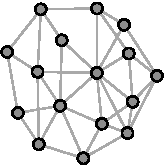
\includegraphics[width=.33\textwidth]{homophNet} & \hspace{2cm} &
  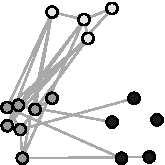
\includegraphics[width=.33\textwidth]{stochEquivNet}  
  \end{tabular}
  \end{table}

  To account for these patterns we can build on what we have so far and find an expression for $\gamma$:
  
  \vspace{-5mm}
  \begin{align*}
  \centering
  y_{ij} &\approx \beta^{T} X_{ij} + a_{i} + b_{j} + \gamma(u_{i},v_{j})
  \end{align*}

}
%%%%%%%%%%%%%%%%%%%%%%%%%%%%%%%%%%%%%%%%%%%%%%%%%%%%%%%%%%%%

%%%%%%%%%%%%%%%%%%%%%%%%%%%%%%%%%%%%%%%%%%%%%%%%%%%%%%%%%%%%
\frame{
  \frametitle{Latent Factor Model: The ``M'' in AME}

Each node $i$ has an unknown latent factor:

\vspace{-5mm}
\begin{align*}
{\textbf{u}_{i},\textbf{v}_{j}} \in \mathbb{R}^{k} \;\; i,j \in \{1, \ldots, n \} \\
\end{align*}

\vspace{-5mm}
The probability of a tie from $i$ to $j$ depends on their latent factors (Hoff 2008, Hoff 2015, Minhas, Hoff \& Ward 2018):

\vspace{-5mm}
\begin{align*}
\begin{aligned}
  \gamma(\textbf{u}_{i}, \textbf{v}_{j}) &= \textbf{u}_{i}^{T} D \textbf{v}_{j} \\
  &= \sum_{k \in K} d_{k} u_{ik} v_{jk} \\
  &D \text{ is a  } K \times K \text{ diagonal matrix}
\end{aligned}
\end{align*}

Can account for both stochastic equivalence and homophily

}
%%%%%%%%%%%%%%%%%%%%%%%%%%%%%%%%%%%%%%%%%%%%%%%%%%%%%%%%%%%%

%%%%%%%%%%%%%%%%%%%%%%%%%%%%%%%%%%%%%%%%%%%%%%%%%%%%%%%%%%%%
\frame{
  \frametitle{AME}

The full AME framework enables us to not only account for the types of dependencies that often arise in dyadic data but also estimate them in a fully Bayesian framework: 

\begin{align}
  \begin{aligned}
    y_{ij} \;=\; f(\theta_{ij}) &\text{, where } \\
    \theta_{ij} \;=\;& \bm\beta_{d}^{\top} \mathbf{X}_{ij} + \bm\beta_{s}^{\top} \mathbf{X}_{i} + \bm\beta_{r}^{\top} \mathbf{X}_{j} \text{\qquad(Exogenous parameters)} \\
    & + a_{i} + b_{j} + \epsilon_{ij} \text{\qquad\qquad\qquad\quad(SRRM parameters)} \\
    & + \mathbf{u}_{i}^{\top} \mathbf{D} \mathbf{v}_{j}  \text{\qquad\qquad\qquad\qquad\qquad\;(LFM parameters)} \\ 
  \label{eqn:ame}
  \end{aligned}
\end{align}

}
%%%%%%%%%%%%%%%%%%%%%%%%%%%%%%%%%%%%%%%%%%%%%%%%%%%%%%%%%%%%

%%%%%%%%%%%%%%%%%%%%%%%%%%%%%%%%%%%%%%%%%%%%%%%%%%%%%%%%%%%%
\frame{
  \frametitle{Simulation}

Assume that the true data-generating process for a particular $Y$ is given by:

\vspace{-8mm}
\begin{align}
  y_{i,j} \sim  \mu + \beta x_{i,j} + \gamma w_{i,j} + \epsilon_{i,j}
  \label{eqn:sim}
\end{align}

We compare inference for $\mu$ and $\beta$---the latter parameter would be of primary concern for applied scholars---using three models:

\begin{itemize}
  \item the ``standard'' international relations approach estimated through a typical generalized linear model; 
  \item the AME approach outlined in the previous section with a unidimensional latent factor space ($K=1$);
  \item and an ``oracle'' regression model that assumes we have measured all sources of dependencies and thus includes both $x_{i,j}$ and $w_{i,j}$. 
\end{itemize}

}
%%%%%%%%%%%%%%%%%%%%%%%%%%%%%%%%%%%%%%%%%%%%%%%%%%%%%%%%%%%%

%%%%%%%%%%%%%%%%%%%%%%%%%%%%%%%%%%%%%%%%%%%%%%%%%%%%%%%%%%%%
\frame{
  \frametitle{Bias Comparison}

We first compare the performance of the models in terms of how well they estimate the true values of $\mu$ and $\beta$:

\vspace{8mm}
\centering
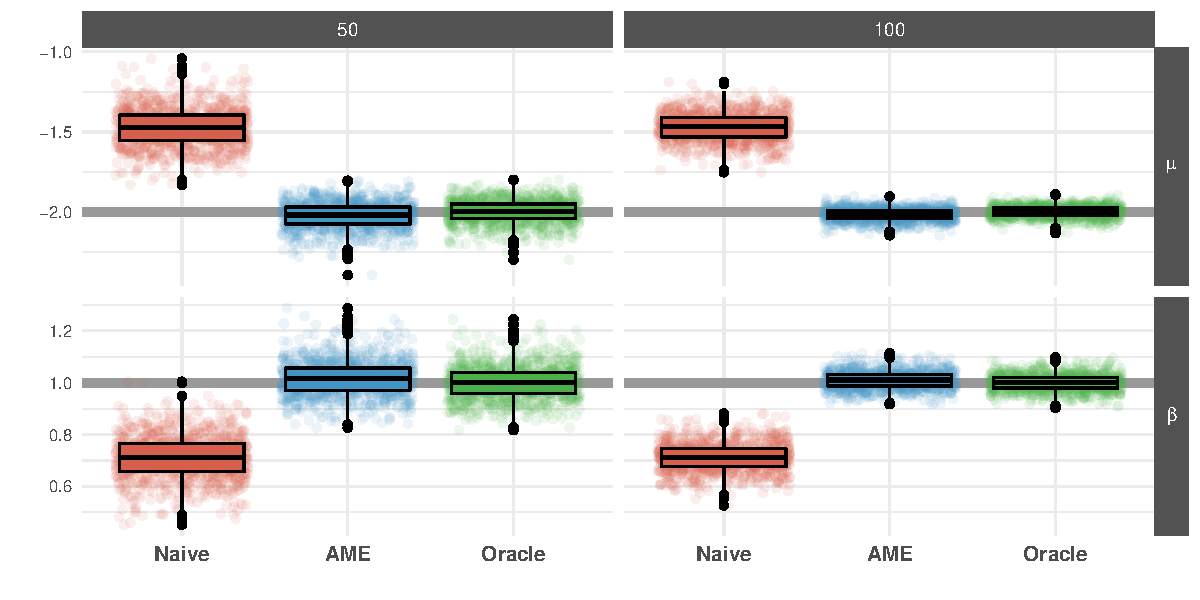
\includegraphics[width=1\textwidth]{ameSimBias_all.pdf}

}
%%%%%%%%%%%%%%%%%%%%%%%%%%%%%%%%%%%%%%%%%%%%%%%%%%%%%%%%%%%%

%%%%%%%%%%%%%%%%%%%%%%%%%%%%%%%%%%%%%%%%%%%%%%%%%%%%%%%%%%%%
\frame{
  \frametitle{Coverage Comparison}

Next, we estimate the 95\% confidence interval for the three models in each of the simulations and estimate the proportion of times that the true value fell within those intervals:

\vspace{8mm}
\centering
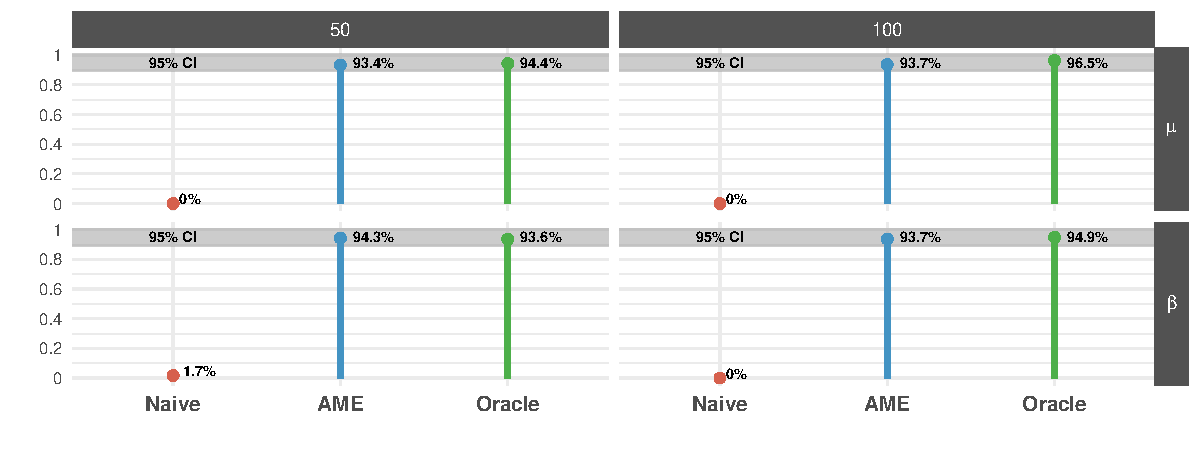
\includegraphics[width=1\textwidth]{ameSimCover_all.pdf}

}
%%%%%%%%%%%%%%%%%%%%%%%%%%%%%%%%%%%%%%%%%%%%%%%%%%%%%%%%%%%%

%%%%%%%%%%%%%%%%%%%%%%%%%%%%%%%%%%%%%%%%%%%%%%%%%%%%%%%%%%%%
\frame{
  \frametitle{What about the missing variable?}

Unobserved dependencies should be captured through the multiplicative effects portion of the model, $\mathbf{U}^{\top} \mathbf{D} \mathbf{V}$:

\vspace{8mm}
\centering
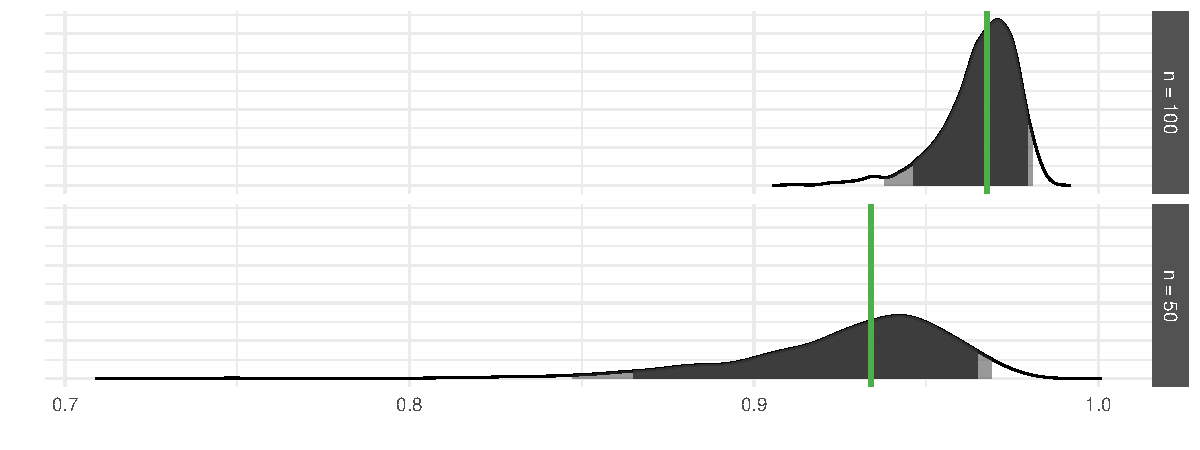
\includegraphics[width=1\textwidth]{ameSimCorr.pdf}

}
%%%%%%%%%%%%%%%%%%%%%%%%%%%%%%%%%%%%%%%%%%%%%%%%%%%%%%%%%%%%

%%%%%%%%%%%%%%%%%%%%%%%%%%%%%%%%%%%%%%%%%%%%%%%%%%%%%%%%%%%%
\frame{
  \frametitle{Empirical Applications}

Descriptive information about the replicated studies: 

\vspace{5mm}
% \footnotesize{
% \begin{tabular}{lccccc}
% 	& Model &  Date Range & N. Actors  & Dyads Type & Clustering $\sigma_{\hat{\beta}}$ \\ \toprule
% 	Reiter \& Stam (2003) & Logit &1945--1995 &  193 & Directed & Robust \\
% 	Weeks (2012) & Logit & 1946--1999 & 197 & Directed & Robust \\
% 	Gibler (2017) & Logit & 1816--2008 & 193 & Undirected & Robust \\ \bottomrule
% \end{tabular}
% }
\begin{tabular}{lcccc}
	& Model &  Date Range & N. Actors  & Dyads Type \\ \toprule
	Reiter \& Stam (2003) & Logit &1945--1995 &  193 & Directed \\ 
	Weeks (2012) & Logit & 1946--1999 & 197 & Directed \\
	Gibler (2017) & Logit & 1816--2008 & 193 & Undirected \\ \bottomrule
\end{tabular}

}
%%%%%%%%%%%%%%%%%%%%%%%%%%%%%%%%%%%%%%%%%%%%%%%%%%%%%%%%%%%%

%%%%%%%%%%%%%%%%%%%%%%%%%%%%%%%%%%%%%%%%%%%%%%%%%%%%%%%%%%%%
\frame{
  \frametitle{Predictive Comparison}

\centering   
\begin{tabular}{lccc}
~ &  Model & AUC (ROC) & AUC (PR) \\ \toprule
\multirow{2}{*}{Reiter \& Stam (2003)} & \cellcolor{blue!10}AME & \cellcolor{blue!10}0.96 & \cellcolor{blue!10}0.15 \\
~ & GLM & 0.92 & 0.08 \\
\multirow{2}{*}{Weeks (2012)} & \cellcolor{blue!10}AME & \cellcolor{blue!10}0.97 & \cellcolor{blue!10}0.15 \\
~ & GLM & 0.64 & 0.00 \\
\multirow{2}{*}{Gibler (2017)} & \cellcolor{blue!10}AME & \cellcolor{blue!10}0.91 & \cellcolor{blue!10}0.08 \\
~ & GLM & 0.52 & 0.00 \\ \bottomrule
\end{tabular}

}
%%%%%%%%%%%%%%%%%%%%%%%%%%%%%%%%%%%%%%%%%%%%%%%%%%%%%%%%%%%%

%%%%%%%%%%%%%%%%%%%%%%%%%%%%%%%%%%%%%%%%%%%%%%%%%%%%%%%%%%%%
\frame{
  \frametitle{Results robust?}

\footnotesize{
\begin{table}[ht]
\centering
  \begin{tabular}{l p{4cm} l} \toprule
    \multirow{2}{*}{Study} & \multirow{2}{*}{Central Finding} &  Confirmed after \\
    & &  accounting for dependencies? \\ \toprule
    Reiter \& Stam (2003) & Personalist Regimes Attack Democracies, Not Vice Versa & {Confirmed} \\ \midrule
    Weeks (2012) & Bosses, Juntas, and Strongmen are more Aggressive, Machines are Not & {Unconfirmed} \\\midrule
    Gibler (2017) & Power Parity at Time of Entry to International System Increases Conflict & {Unconfirmed}\\ \bottomrule
  \end{tabular}
\end{table}
}

}
%%%%%%%%%%%%%%%%%%%%%%%%%%%%%%%%%%%%%%%%%%%%%%%%%%%%%%%%%%%%

%%%%%%%%%%%%%%%%%%%%%%%%%%%%%%%%%%%%%%%%%%%%%%%%%%%%%%%%%%%%
\frame{
  \frametitle{What else did we learn? Reiter \& Stam (2003)}

\begin{tabular}{cc}
  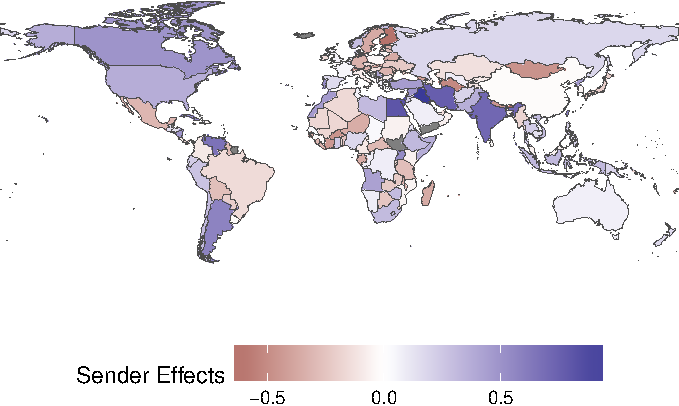
\includegraphics[width=.7\textwidth]{reiter_stam_aEff_map.pdf} &
  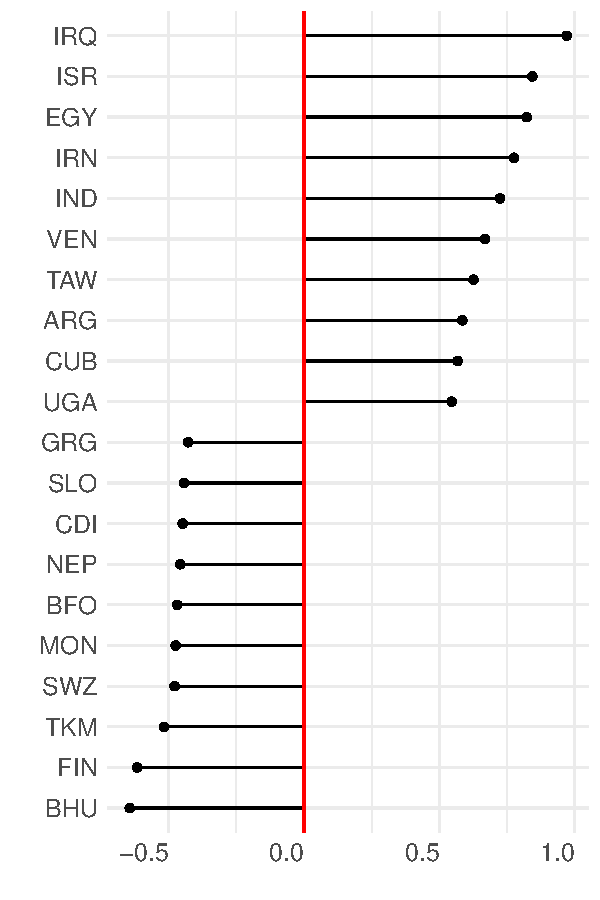
\includegraphics[width=.3\textwidth]{reiter_stam_aEff_line.pdf} \\
\end{tabular}

}
%%%%%%%%%%%%%%%%%%%%%%%%%%%%%%%%%%%%%%%%%%%%%%%%%%%%%%%%%%%%

%%%%%%%%%%%%%%%%%%%%%%%%%%%%%%%%%%%%%%%%%%%%%%%%%%%%%%%%%%%%
\frame{
  \frametitle{What else did we learn? Weeks (2012)}

\centering
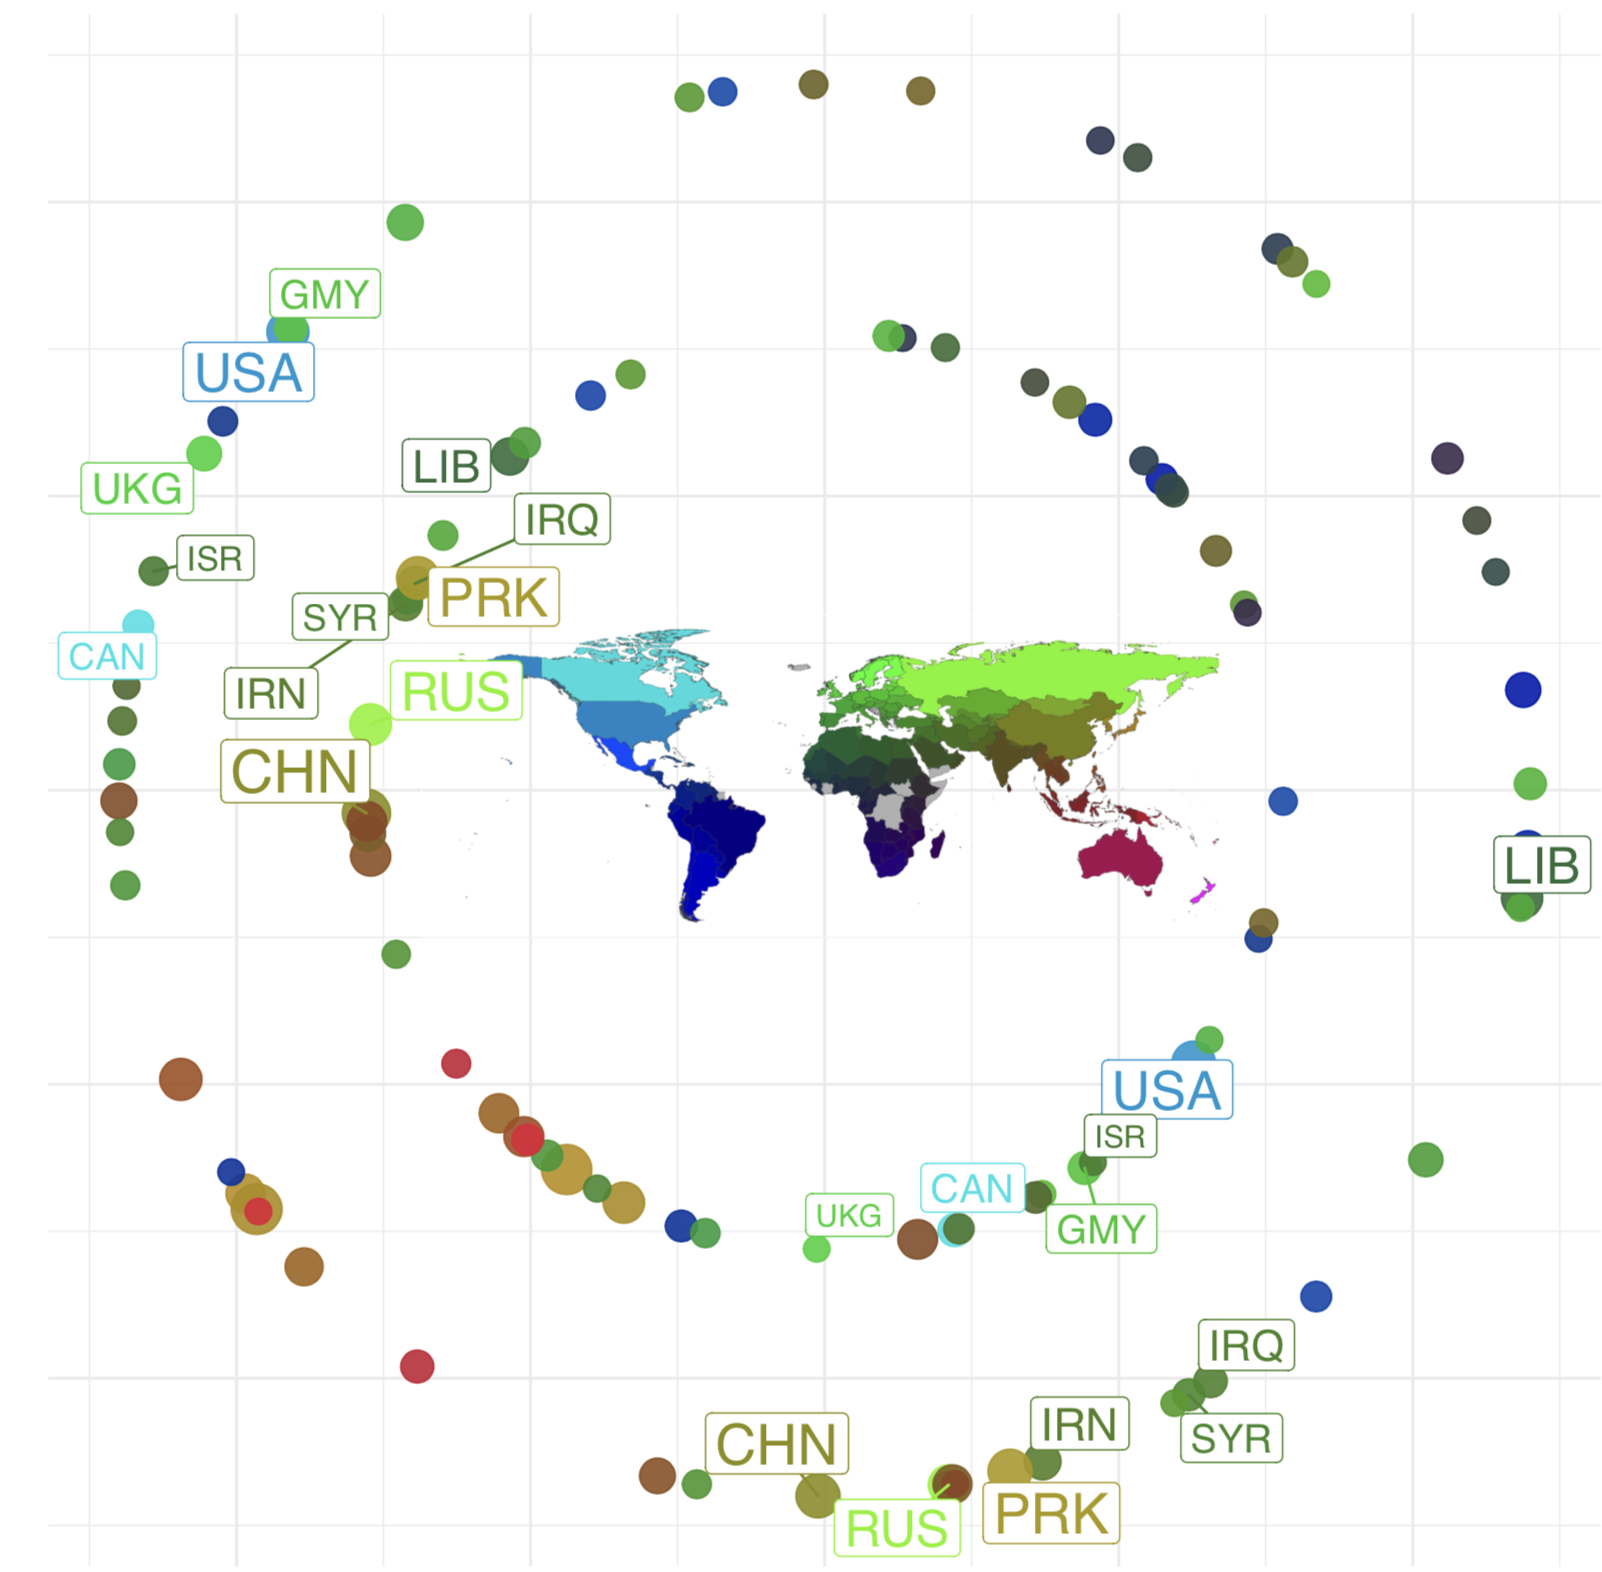
\includegraphics[width=.7\textwidth]{weeks_circPlot.png}

}
%%%%%%%%%%%%%%%%%%%%%%%%%%%%%%%%%%%%%%%%%%%%%%%%%%%%%%%%%%%%

%%%%%%%%%%%%%%%%%%%%%%%%%%%%%%%%%%%%%%%%%%%%%%%%%%%%%%%%%%%%
\frame{
  \frametitle{What else did we learn? Gibler (2017)}

\centering
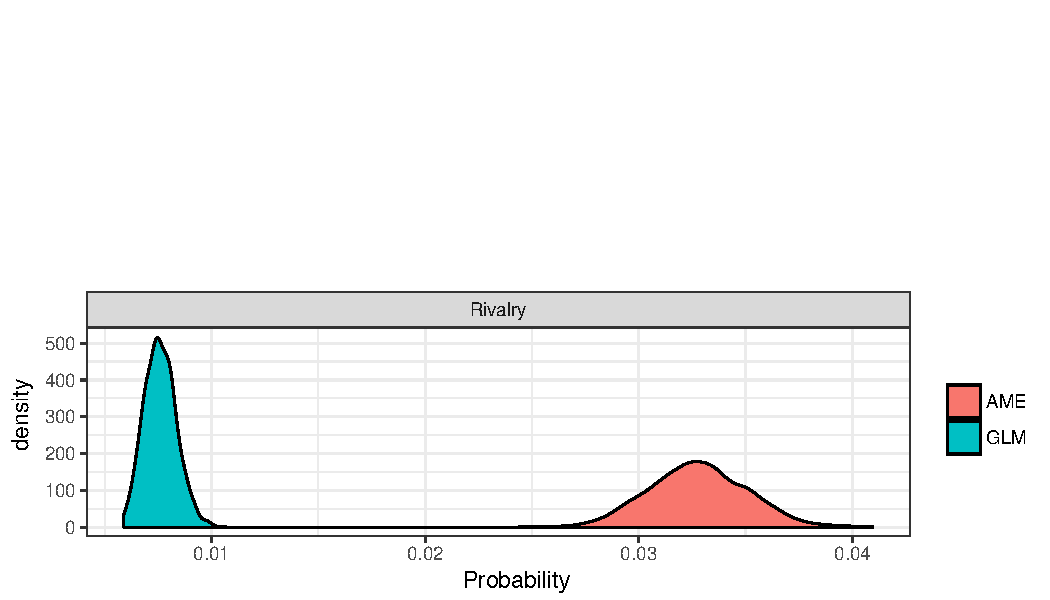
\includegraphics[width=\textwidth]{gibler_margeff.pdf}

}
%%%%%%%%%%%%%%%%%%%%%%%%%%%%%%%%%%%%%%%%%%%%%%%%%%%%%%%%%%%%

%%%%%%%%%%%%%%%%%%%%%%%%%%%%%%%%%%%%%%%%%%%%%%%%%%%%%%%%%%%%
\frame{
\frametitle{Next steps}

\begin{itemize}
	\item Dealing with time varying dependence structure
	\item Parsing out formation, persistence and dissolution
	\item Many other extensions (bipartite, endogenous multilayer networks, ...)
	\item Computational issues ... Bayesian models take time to converge 
\end{itemize}
}
%%%%%%%%%%%%%%%%%%%%%%%%%%%%%%%%%%%%%%%%%%%%%%%%%%%%%%%%%%%%

% %%%%%%%%%%%%%%%%%%%%%%%%%%%%%%%%%%%%%%%%%%%%%%%%%%%%%%%%%%%%
% \frame{
%   \frametitle{What's Next?}
%
%   \begin{itemize}
%     \item
%   \end{itemize}
%
% }
% %%%%%%%%%%%%%%%%%%%%%%%%%%%%%%%%%%%%%%%%%%%%%%%%%%%%%%%%%%%%

%%%%%%%%%%%%%%%%%%%%%%%%%%%%%%%%%%%%%%%%%%%%%%%%%%%%%%%%%%%%
\plain{Thanks.}
%%%%%%%%%%%%%%%%%%%%%%%%%%%%%%%%%%%%%%%%%%%%%%%%%%%%%%%%%%%%

%%%%%%%%%%%%%%%%%%%%%%%%%%%%%%%%%%%%%%%%%%%%%%%%%%%%%%%%%%%%
\frame{
  \frametitle{Predictive Comparison: Reiter \& Stam (2003)}

\centering
\begin{tabular}{lr}
  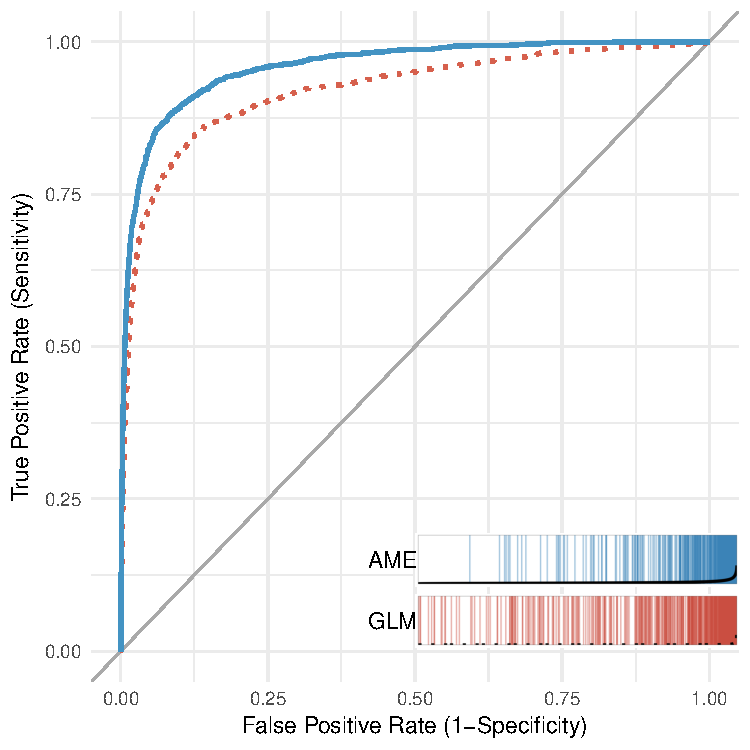
\includegraphics[width=.45\textwidth]{reiter_stam_roc_outSample.pdf} & 
  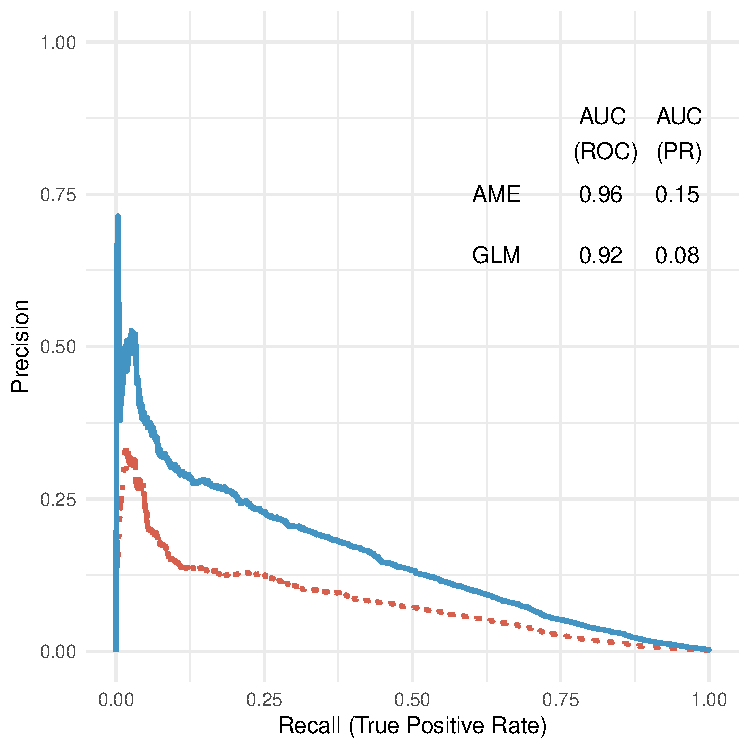
\includegraphics[width=.45\textwidth]{reiter_stam_pr_outSample.pdf} \\
\end{tabular}

}
%%%%%%%%%%%%%%%%%%%%%%%%%%%%%%%%%%%%%%%%%%%%%%%%%%%%%%%%%%%%

%%%%%%%%%%%%%%%%%%%%%%%%%%%%%%%%%%%%%%%%%%%%%%%%%%%%%%%%%%%%
\frame{
  \frametitle{Predictive Comparison: Weeks (2012)}

\centering
\begin{tabular}{lr}
  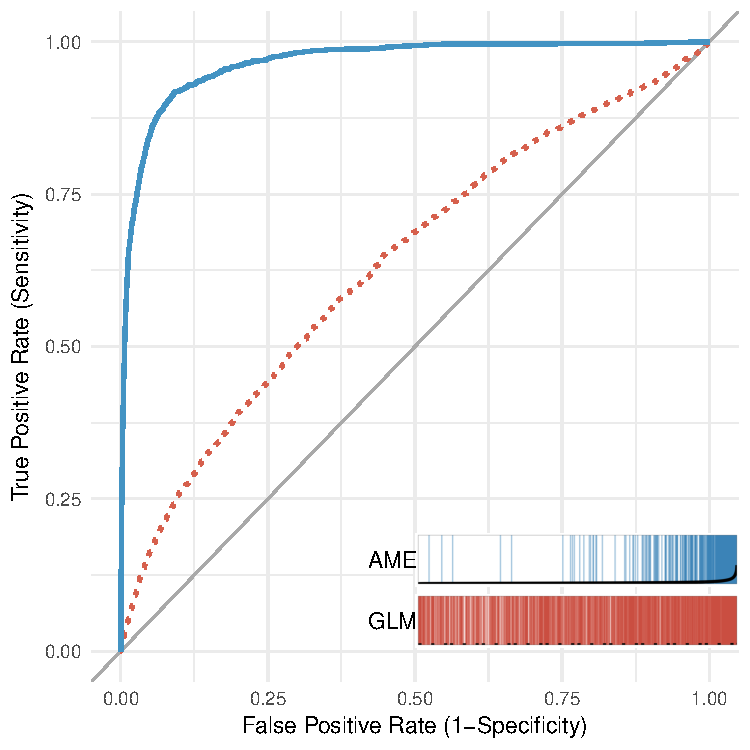
\includegraphics[width=.45\textwidth]{weeks_roc_outSample.pdf} & 
  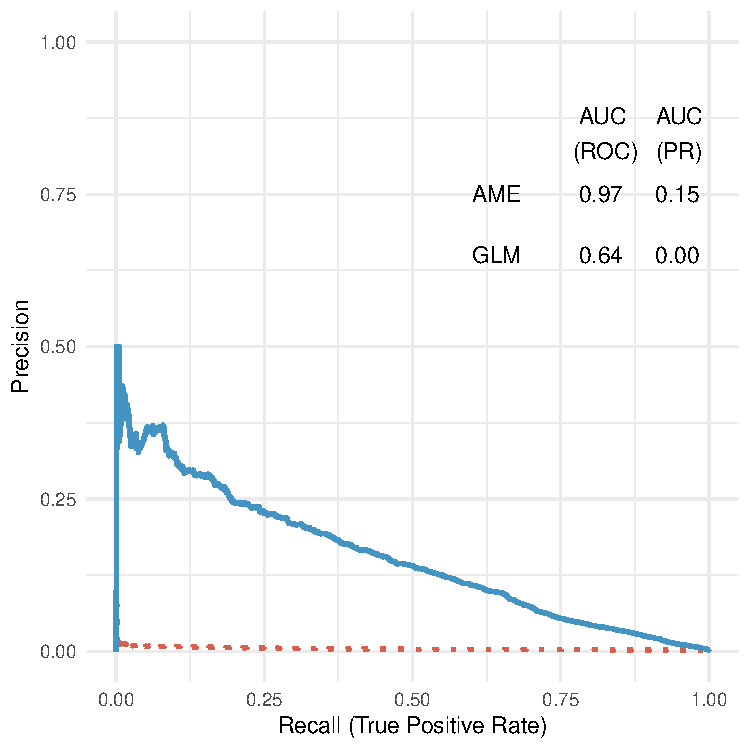
\includegraphics[width=.45\textwidth]{weeks_pr_outSample.pdf} \\
\end{tabular}

}
%%%%%%%%%%%%%%%%%%%%%%%%%%%%%%%%%%%%%%%%%%%%%%%%%%%%%%%%%%%%

%%%%%%%%%%%%%%%%%%%%%%%%%%%%%%%%%%%%%%%%%%%%%%%%%%%%%%%%%%%%
\frame{
  \frametitle{Predictive Comparison: Gibler (2017)}

\centering
\begin{tabular}{lr}
  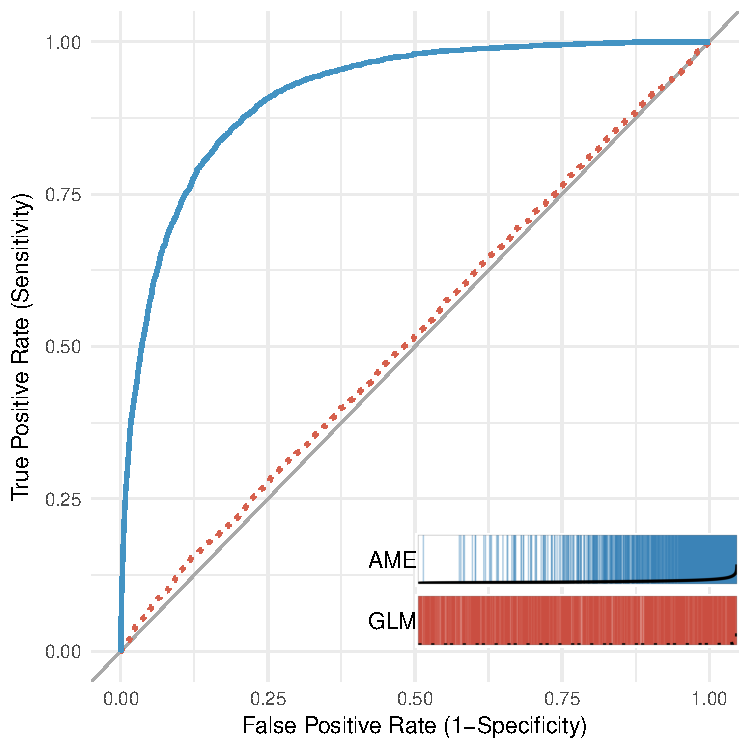
\includegraphics[width=.45\textwidth]{gibler_roc_outSample.pdf} & 
  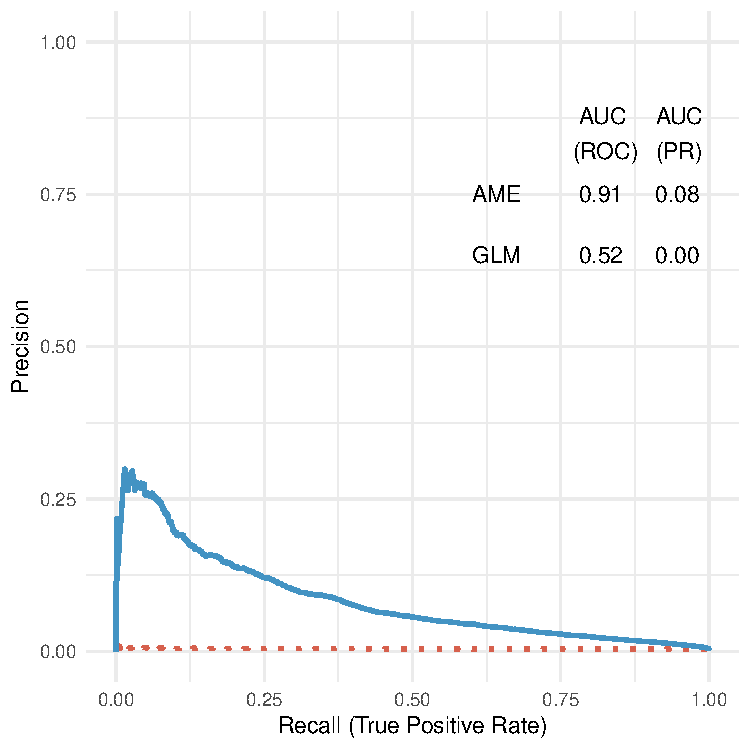
\includegraphics[width=.45\textwidth]{gibler_pr_outSample.pdf} \\
\end{tabular}

}
%%%%%%%%%%%%%%%%%%%%%%%%%%%%%%%%%%%%%%%%%%%%%%%%%%%%%%%%%%%%

\end{document}
